\documentclass{article}
\usepackage{float}
\usepackage{graphicx}
\graphicspath{ {images/} }

\title{DSP Project Report: ECG Signal Analysis}
\author{Abhinav Chawla (IMT2013002) \\ Apoorv Vikram Singh (IMT2013006) \\ Rishabh Bhadauria (IMT2013034) \\ Shivam Kumar (IMT2013042) \\Siddartha Sekhar Padhi (IMT2013043) \\ Ujjwal Jain (IMT2013056) }
\date{\today}

\begin{document}

\maketitle

\section{Introduction}
Electrocardiogram (ECG) is a nearly periodic signal that reflects the activity of the
heart. A lot of information on the normal and pathological physiology of heart can be
obtained from ECG. However, the ECG signals being non-stationary in nature, it is very
difficult to visually analyze them. Thus the need is there for computer based methods for
ECG signal Analysis. \\ \\
We were given the ECG data collected using the Wipro AssureHealth device doing
various physical activities. The sampling frequency was 250Hz. The data given to
us didn't look like an ideal ECG which we generally see in the hospitals. The
sources for additional noise could be powerline interference, electrode contact
noise , the baseline drift and motion artifacts. There could be EMG from the
chest wall. There also could be instrumentation noise. \\ \\
The purpose of this report is to analyse the data and make a C code such that
the output could be given in real-time. 

\section{Data Analysis}
First we analysed the frequency spectrum of the plots given. The signal we
received. The frequency in Hertz was only from 0 to 25 Hz, as can be seen from
the figure. \\
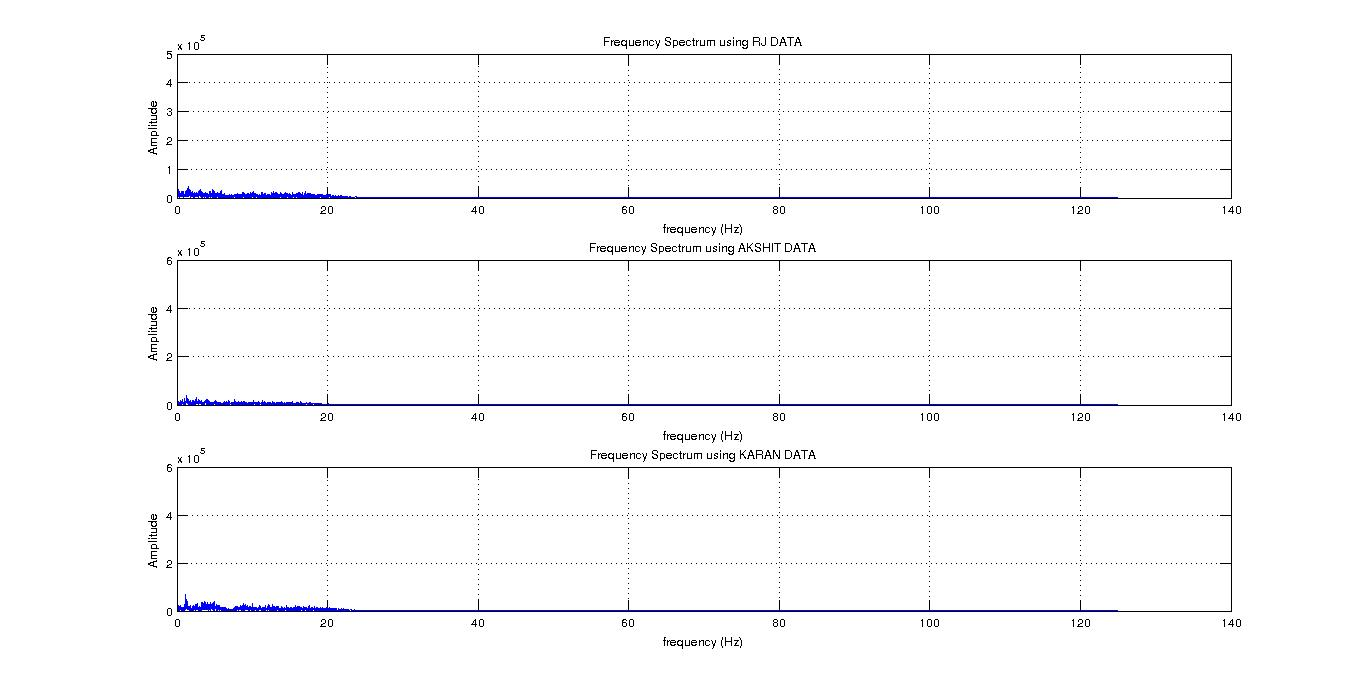
\includegraphics[width=\textwidth]{freq} \\ \\ 
The raw data given to us was told to be baseline filtered signal and the cleaned
signal is the raw signal passed through a bandpass filter. As seen from the
frequency spectrum there is no powerline interference as there is no frequency
of 50Hz and multiple of 50Hz. To remove the powerline interference we can use
a notch filter to remove 50Hz and it's multiple frequencies, that is, 50Hz and
100Hz.\\ \\
However, as per the plot, the signal was not baseline corrected. After
subtracting the signal from it's amplitude mean, we get baseline corrected
signal. This gives us a similar plot as passing the signal from a bandpass
filter, allowing the frequency between 10Hz and 20Hz. \\ \\
The plot here plots the original signal in red, the mean subtraction data is in
blue and the bandpass filter data is in green. \\ 
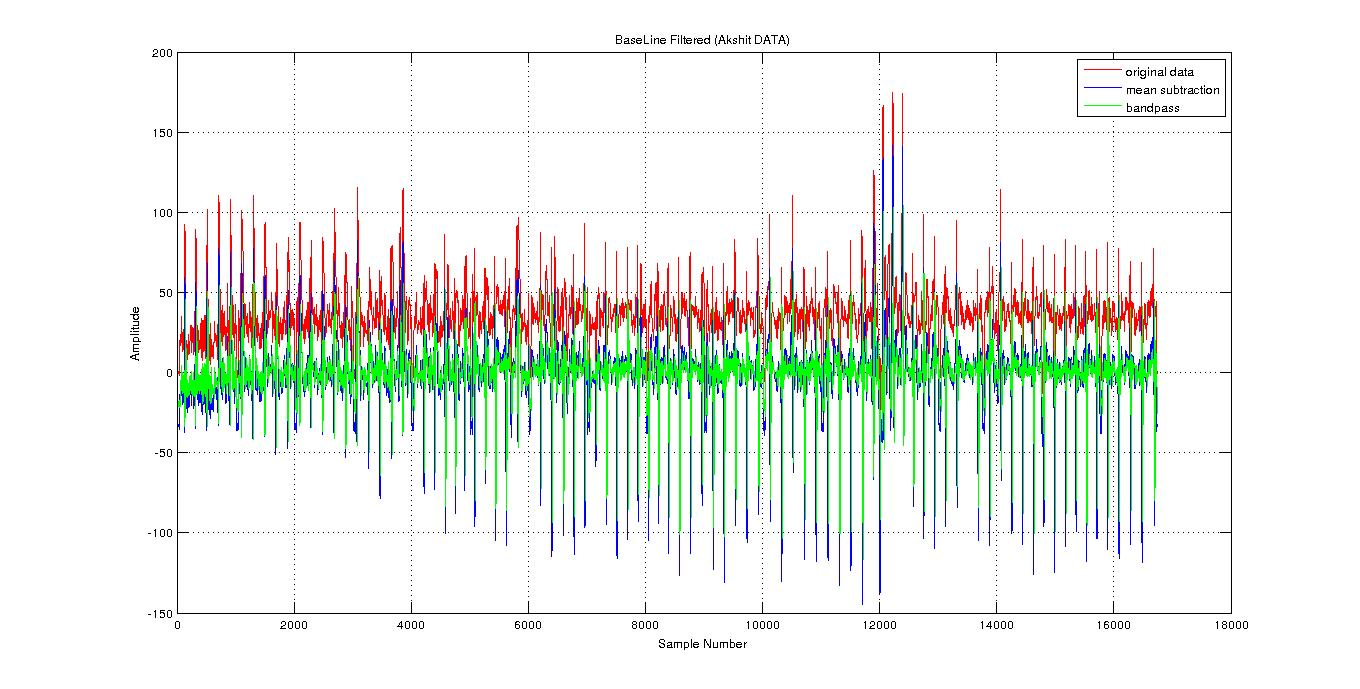
\includegraphics[width=\textwidth]{baseline}  \\ \\
For the R-peak detection, after filtering we double differentiated the data, the
basic purpose of which was to amplify the noise. Here the noise in our case can
be thought of as the R-peak. So if there is any peak, it will amplify those.
When subtracting 2 points nearby; if they are close to each other, the points
will suppress, and if they are apart from each-other they will get amplified.
After that we took an optimal window size of 175 samples (found after
exploratory analysis), and found the peaks in the data. \\ \\ 
The original data can be seen and double differentiated data also can be seen
from the plot to clearly see the peaks. We didn't use any threshold as it can be 
misleading, due to varying thresholds. Instead, a maximum was found in every
window, given the values are not zero.\\
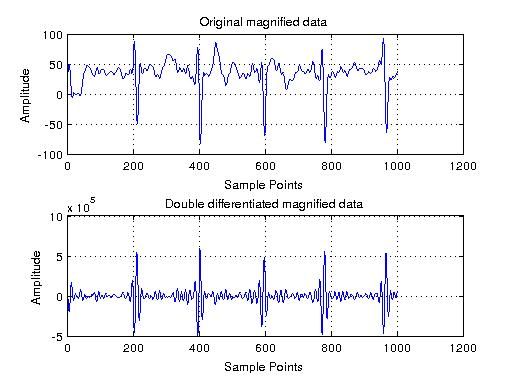
\includegraphics[width=\textwidth]{doublediff}
\section{Code}
The code for bandpass, bandstop, peak detection and a simple baseline removal 
(by removing amplitudes mean from the amplitude) is written in C. The bandstop filter
can act as a notch filter to remove the powerline interference. The bandpass can act as
both high-pass and low-pass by adjusting the values in the code. \\ \\ 
Assumption taken is that in the input file, we don't get more than $10^5$ sample points
($\approx$ 6 minutes), and also in those 6 minutes, a normal functioning person using the
Wipro AssureHealth would not have more than 1000 heart beats. 
\subsection{Coding Environment}
The code was written in C, and compiled using the gcc compiler (version 4.9.3), in the
Ubuntu 14.04 Operating System. The plots were generated using Matlab 2013a. The report 
is written in \LaTeX, and compiled using pdfTeX 3.1415926-2.5-1.40.14 (TeX Live 2013/Debian).

\begin{thebibliography}{9}
\bibitem{stanford} 
Xiao HU , Zhong XIAO and Ni ZHANG 
\textit{Removal of baseline wander from ECG signal based on a statistical weighted moving average filter *}. 
\\\texttt{www.zju.edu.cn/jzus/opentxt.php?doi=10.1631/jzus.C1010311}
 
 \bibitem{einstein} 
 Hossein Rabbani, M. Parsa Mahjoob, E. Farahabadi and A. Farahabadi
 \textit{R Peak Detection in Electrocardiogram Signal Based on an Optimal Combination of Wavelet Transform, Hilbert Transform, and Adaptive Thresholding}
 \\\texttt{http://www.ncbi.nlm.nih.gov/pmc/articles/PMC3342622/}

 \bibitem{knuthwebsite} 
 Finite Impulse Response (FIR) Filter \textit{Digital Filter Design}, reterieved from
 \texttt{http://www.mikroe.com/chapters/view/72/chapter-2-fir-filters/}
 \end{thebibliography}
\end{document}
